\documentclass[a5paper,ngerman,xcolor=dvipsnames]{scrartcl}
\usepackage{fontspec}
\setmainfont[Mapping=tex-text]{Vollkorn}
\setsansfont[Mapping=tex-text]{Vollkorn}
\setmonofont{Vollkorn}
\PassOptionsToPackage{normalem}{ulem}
\usepackage{ulem}
\usepackage{tikz}
\usetikzlibrary{positioning,fadings,through}
\usetikzlibrary{patterns}
\definecolor{balken}{HTML}{bbbbbb}
\definecolor{balken_border}{HTML}{888888}

\usepackage{enumitem,amssymb}
\usepackage{wasysym}
\usepackage{xcolor}
\usepackage{eso-pic}
\usepackage{multicol}
\usepackage{soul}
\setul{0.3ex}{0.5ex}
\setulcolor{magenta}

\usepackage{graphicx}
\graphicspath{ {images/} }

\pagestyle{empty}
\usepackage[left=1.5cm,right=1.5cm,top=0.5cm,bottom=0.5cm,includeheadfoot]{geometry}
\renewcommand*{\sectionformat}{}
\setlength{\parindent}{0pt}

\usepackage{xunicode}
\usepackage{polyglossia}
\setdefaultlanguage[variant=german,spelling=new,babelshorthands=true]{german}
\begin{document}
{%
\Huge
\begin{center}
\ul{\textbf{Bierschnitzeljagd}}
\end{center}
}%

\vspace{2em}

\noindent\textbf{Regeln:} Jedes Team sammelt möglichst viele Punkte, gemäß der Liste
unten. Nehmt die Punkte nicht (bier-)ernst. \textbf{Ziel} ist es, möglichst viel von der
Stadt und (Hefe-)Kultur kennenzulernen.

\begin{enumerate}
\setlength\itemsep{0.3em}
\item Möglichst viele verschiedene Biere von vielen Brauerein einsammeln. (Dokumentation mit voll ausgefüllten Bierbogen, 1$\times$ Punkt pro Bier, pro Rauchbier $+1\times$ Punkt extra)
\item Bamberger Hörnla essen. (1$\times$ Punkt pro Hörnla; die Besten gibt's beim Bäcker Seel, da gibt's jeweils 1$\times$ Extrapunkt)
\item 1$\times$ Paar Bamberger Bratwürste gegessen. (2x Punkte)
\item 1$\times$ Bamberger Zwiebel gegessen. (2x Punkte)
\item 1$\times$ Schäufela gegessen. (2x Punkte)
\item »A U« oder ein »Spezi« bestellt. (je 3$\times$ Punkte, zählt je nur einmal)
\item Glühwein auf dem Weihnachtsmarkt trinken (je 1$\times$ Punkt)
\item Traditionelle Keller und Brauereien besucht (je 3$\times$ Punkte):
    \begin{multicols}{2}
    \begin{itemize}
    \item \emph{Einhornkeller}
    \item \emph{Stöhrenkeller}
    \item \emph{Spezialkeller}
    \item \emph{Bootshaus}
    \item \emph{Sternla}
    \item \emph{Schlenkerla}
    \item \emph{Mahr's Bräu}
    \item \emph{Brauerei Fässla}
    \item \emph{Brauerei Keesmann}
    \item \emph{Brauereigasthof Spezial}
    \item \emph{Brauerei Ambräusianum}
    \item \emph{Klosterbräu}
    \item \emph{Landwehrbräu}
    \item \emph{Brauerei Greifenklau}
    % \item Ahörnla % Besuchen wir eh abends.
    \end{itemize}
    \end{multicols}

\vspace{1em}
\begin{center}\footnotesize\emph{(Bitte wenden)}\end{center}
\newpage
\item Sehenswürdigkeiten (nur einmal vergebbar, Dokumentation mit Gruppenbild in der Signalgruppe):
    \begin{multicols}{2}
    \begin{itemize}
    \setlength\itemsep{0em}
    \item \emph{Rosengarten} (2$\times$ Punkte)
    \item \emph{Altenburg} (5$\times$ Punkte)
    \item \emph{Theresienhain} (1$\times$ Punkte)
    \item \emph{Dom} (1$\times$ Punkt)
    \item \emph{Michelsberg} (2$\times$ Punkt)
    \item \emph{Altes Rathaus} (1$\times$ Punkt)
    \item \emph{Klein Venedig} (1$\times$ Punkt)
    \item \emph{Gabelmoo} (1$\times$ Punkt)
    \item \emph{Apfelweibla} (2$\times$ Punkt)
    \item \emph{Bamberger Reiter} (1$\times$ Punkt)
    \end{itemize}
    \end{multicols}
\end{enumerate}

Der Arbeitskreis Wochenende
(\textbf{\textcolor{red}{A}\textcolor{green}{K}\textcolor{blue}{W}}) wünscht viele
Fußpilse, Erfolg und vor allem Spaß.  Seid dabei bitte vernünftig und trinkt
nicht mehr als ihr vertragt: Kotzen wird nämlich mit Minuspunkten bestraft.

\vspace{2em}

Coole Teams denken sich übrigens auch einen Namen für sich aus.
Für das Team mit den meisten Punkten ist zudem \ul{ein Preis} vorgesehen.

\vspace{2em}
\begin{center}
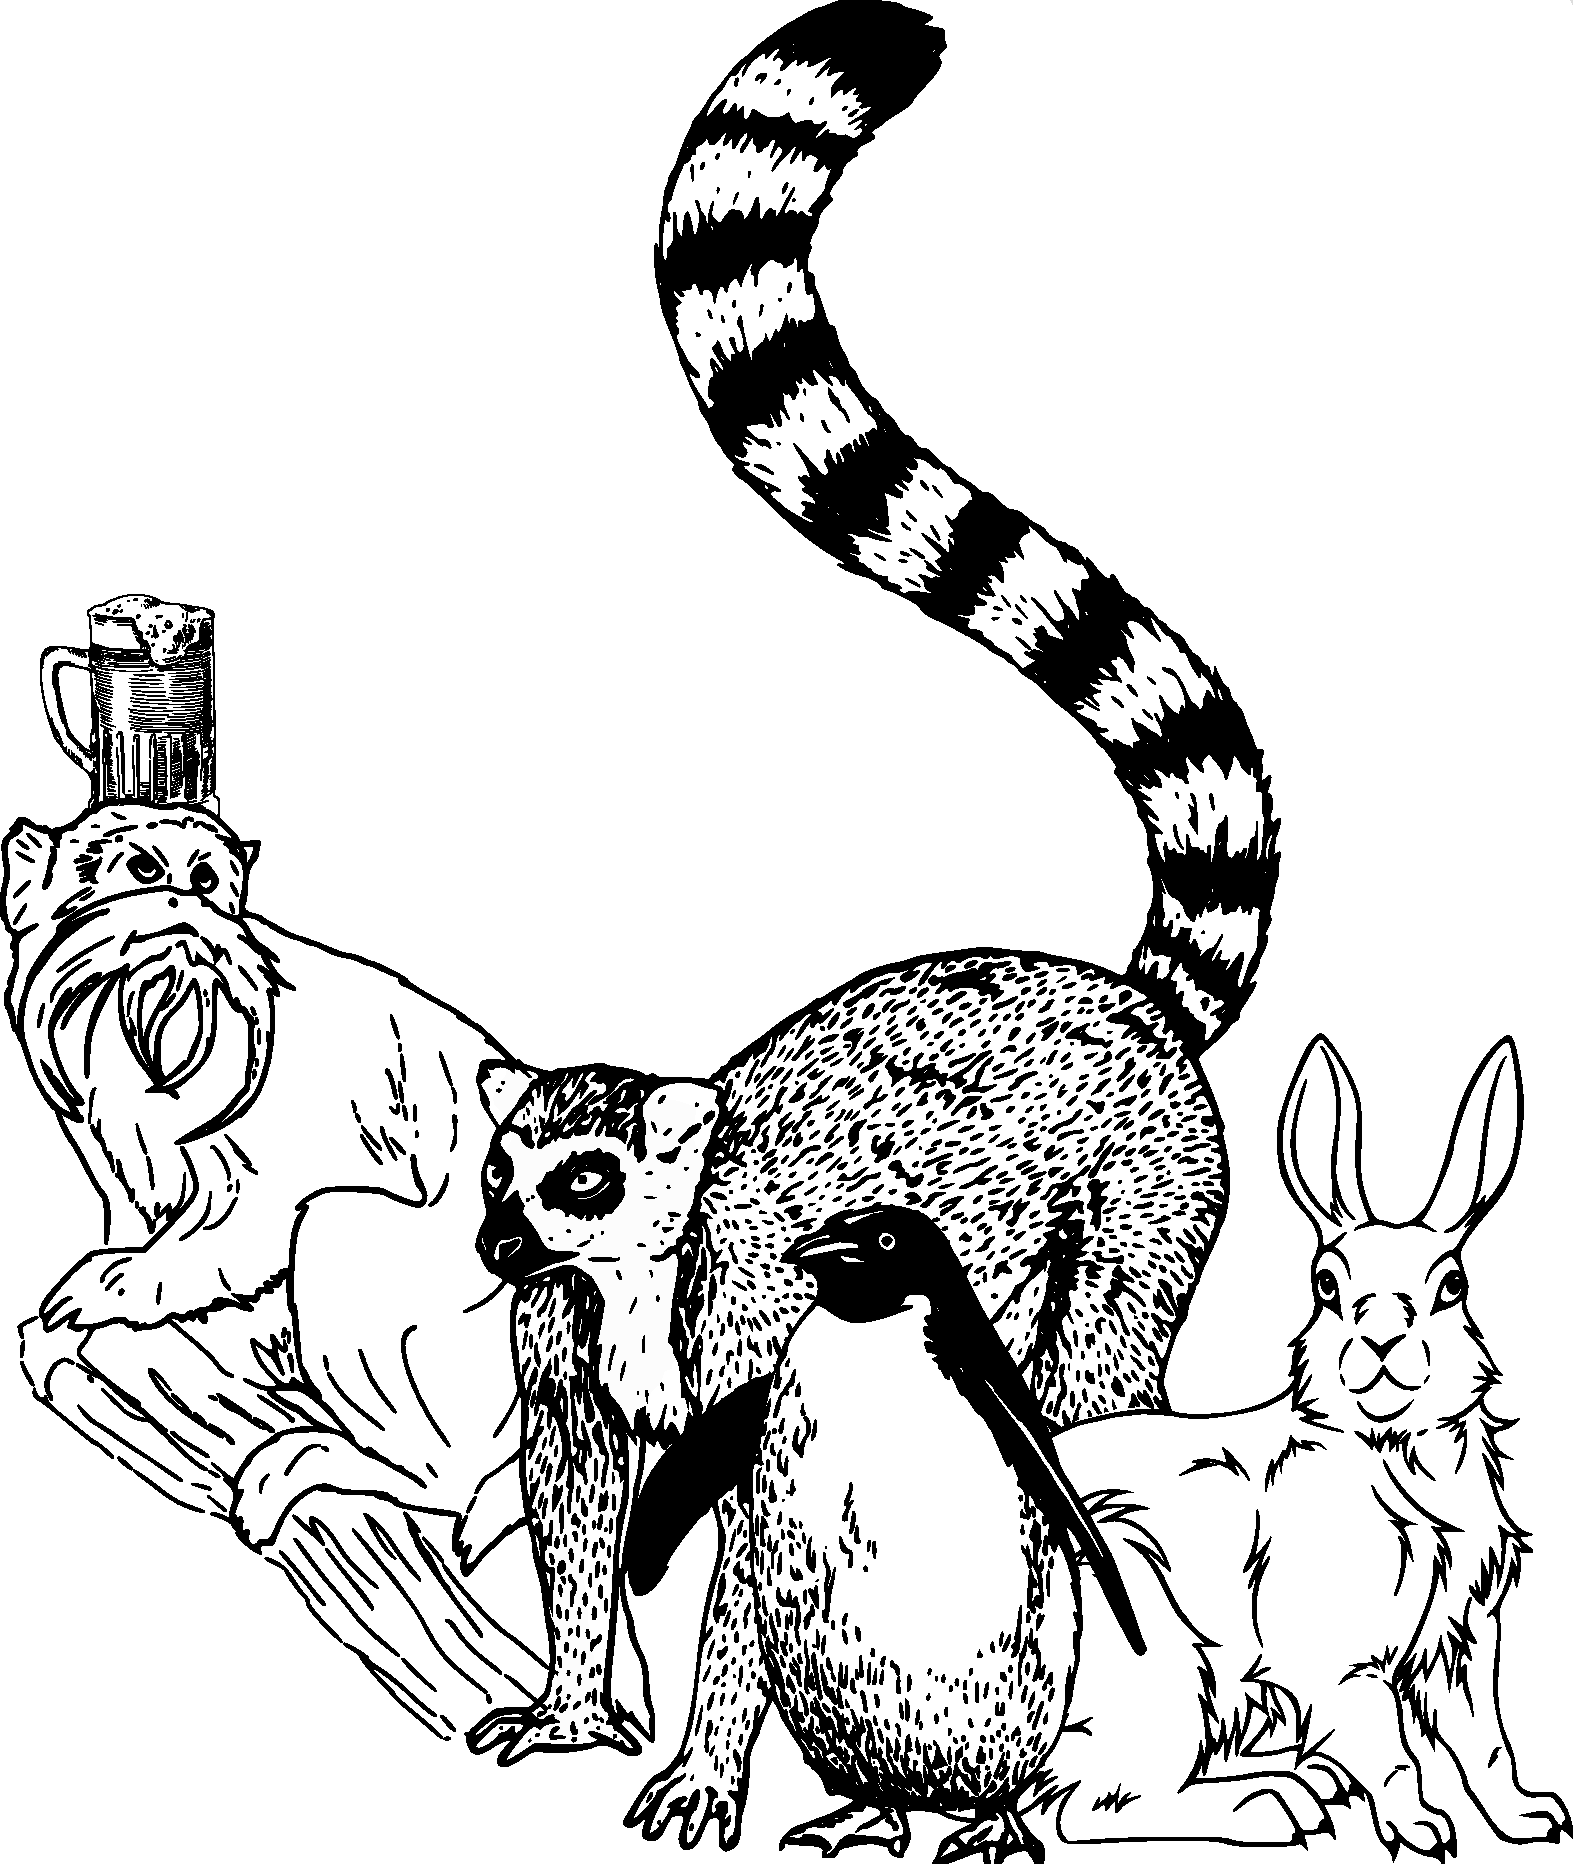
\includegraphics[scale=0.25]{akw.pdf}
\end{center}

\end{document}
